\documentclass[11pt, a4paper]{article}

\usepackage{amsmath}
\usepackage{amsfonts} %Matheschriften
\usepackage{amssymb} %Mathesymbole
%\usepackage{mathptmx} % Einstellung für Schriften und Sonderzeichen in mathematischen Umgebungen
                        % ändert SChriftfont
\usepackage{wasysym} % Stellt diverse Sonderzeichen bereit
\usepackage{siunitx}
\usepackage{float}
\usepackage{microtype}
\usepackage{graphicx}
\usepackage{hyperref}
\usepackage{xcolor}
\usepackage[section]{placeins}


\usepackage[ngerman]{babel}
\addto\captionsngerman{%
 \renewcommand{\abstractname}{Einleitung}}

\title{Versuch 4: Pohlsches Rad}
\author{Jascha Fricker, Benedict Brouwer}

\begin{document}
    \maketitle

    

    \begin{abstract}
        In diesen Versuch wird ein gedämpfter harmonischer Oszillator untersucht. Harmonische Oszillatoren
        sind ein wichtiges Modell in der Physik, da sie sehr viele Systeme in der realen Welt beschreiben können.
        Ein berühmtes Thema sind z. B. Resonanzkatastrophen, bei dehnen große Bauwerke in ihrer Eingenschwingung
        angeregt werden. Genau solche Schwingungen eines getriebenen Harmonischen Oszillators werden auch in diesem
        Versuch untersucht.
    \end{abstract}

    \tableofcontents

    \newpage

    \section{Stromabhängigkeit der Dämpfungskonstanten}
    \subsection{Theorie}
    Je nachdem wie stark ein harmonischer Oszillator gedämpft wird, ändert sich seine Schwingfrequenz.
    Ein gedämpfter harmonischer Oszillator hat die Bewegungsgleichung
    \begin{align}
        \varphi(t) = \varphi_0 \cdot exp(-\lambda t) \cdot cos(\omega_d - \beta), \label{theo5}
    \end{align}
    mit Kreisfrequenz 
    \begin{align} \label{otheo}
        \omega_d = \sqrt{\frac{k}{\Theta} - \lambda^2}
    \end{align} 
    (Drehmoment $\Theta$ und Federkonstante $k$)
    und $\beta$ als Phasenverschiebung. Diese kann aus der Differentialgleichung der Kräfte 
    hergeleitet werden (siehe Aufgabenblatt \cite[(5)]{POR}).
    Bei der in diesem Experiment benutzten Wirbelstrombremse ist die
    Dämpfungskonstante $\lambda$ proportional zum Quadrat des Stroms $I$ durch die Bremse.
    \begin{align} \label{dtheo}
        \lambda = \kappa \cdot I^2.
    \end{align}
    mit $\kappa$ als Proportionalitätsfaktor.

    \subsection{Experimenteller Aufbau}
    Die Stromstärke der Wirbelstrombremse wurde mit einem Labornetzteil eingestellt und
    mit einem VC130 Multimeter gemessen. Nachdem das Pohlsche Rad fast maximal ausgelenkt worden war, 
    wurde der Winkel des Pohlschen Rades abhängig von der Zeit
    mit einem Hall Sensor gemessen und direkt digital aufgenommen.

    \subsection{Auswertung}
    Um die Eingenfrequenz und Dämpfungskonsante abhängig von der Stromstärke zu bestimmen,
    wurde auf jede Messreihe einzeln die Theoriekurve \ref{theo5} mit
    der Funkion \textsf{optimize.curve\_fit} der Pythonbibliothek scipy
    gefittet und auch die Unsicherheit ausgerechnet. Mit diesen 2x15 Datenpunkten können jetzt die Zusammenhänge
    zwischen $\omega_d, \lambda$ und $I$ untersucht werden.


    \subsection{Ergebnisse}
    \begin{figure}
        \centering
        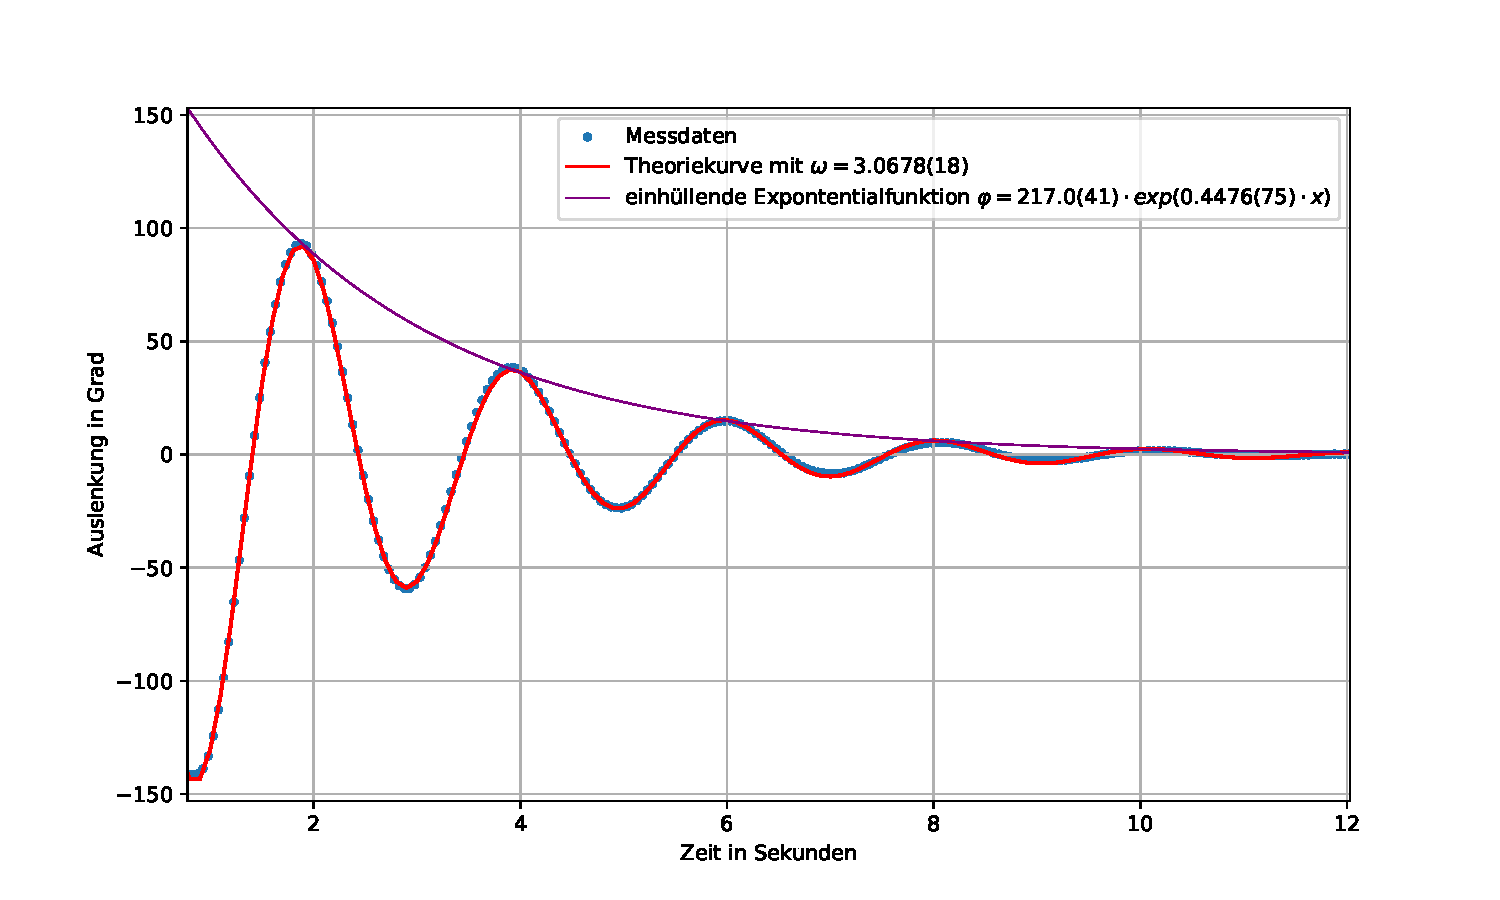
\includegraphics[width=\textwidth]{./6fits.pdf}

        \caption{Beispielmessung}
        \label{fig:beis}
    \end{figure}
    \begin{figure}
        \centering
        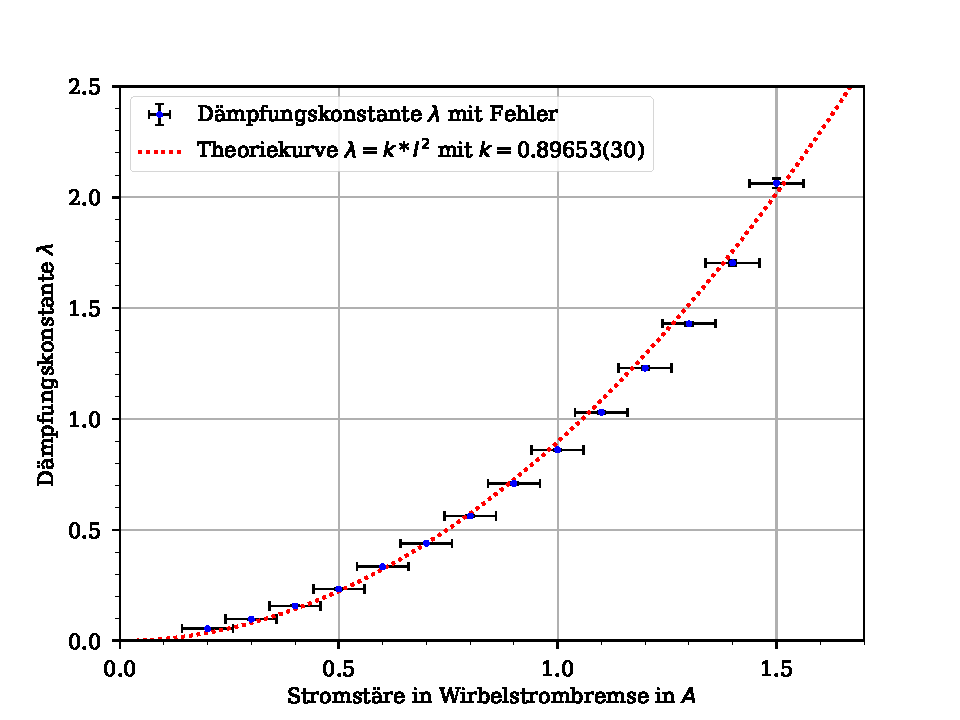
\includegraphics[width=\textwidth]{./6Plot.pdf}

        \caption{Berechung der Dämpfungskonstanten}
        \label{fig:daempf}
    \end{figure}
    \begin{figure}
        \centering
        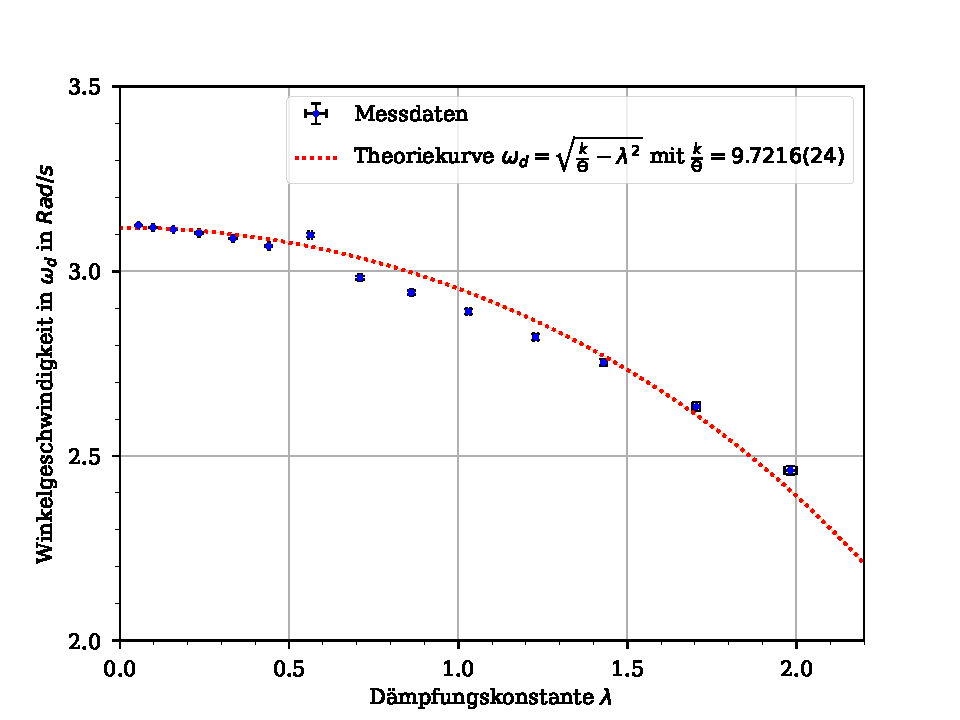
\includegraphics[width=\textwidth]{./7Plot.pdf}

        \caption{Verhältnis Dämpfung und Winkelgeschwindigkeit}
        \label{fig:wink}
    \end{figure}

    In Graph \ref{fig:beis} ist beispielhaft gezeigt, wie die Messdaten und die gefittete Theoriekurve aussehen.
    Die ausgelesenen Dämfungskonstanten wurden in Graph \ref{fig:daempf} gegen die Dämpfungsstromstärke geplottet und mit der
    Theoriekurve (\ref{dtheo}) gefittet. Für die Berechung wurden nur die Fehler der Fits berücksichtigt.
    Im Graph \ref{fig:wink} wurden die ausgelesenen Winkelgeschwindigkeiten gegen die Dämpfung geplottet und mit der Theoriekurve
    (\ref{otheo}) gefittet. Insgesamt wurde ein Proportionalitätsfaktor $\kappa  = 0.89653(30)$ zwischen Dämpfungskonstante und
    Dämpfungsstromstärke und ein Quotien $ \frac{k}{\Theta} = 9.7216(24)$ ermittelt.
   
    \section{Schwingungsverhalten bei gegebener Dämpfung}
    \subsection{Theorie}

    Bei gegebener Dämpfung hat der Oszillator eine charakteristische Eigenfrequenz.
    Die Eigenfrequenz eines Oszillators lässt sich mithilfe der Schwingungsperiode $T$ berechnen
    \begin{align}
        \omega_d = \frac{2\pi}{T}
    \end{align}

    Bei einer gedämpften Schwingung hat die Bewegungsgleichung
    \begin{align}
        \varphi(t) = \varphi_0 \cdot exp(-\lambda t) \cdot cos(\omega_d - \beta), \label{theo}
    \end{align}
    deshalb liegen alle Maxima der Ausschläge des Pohlschen Rades auf der einhüllenden Exponentialfunktion
    \begin{align}
        \varphi(t_n) &= \varphi_0 \cdot exp(-\lambda t_n).
    \end{align}
    Die Abklingzeit
    \begin{align}
        \tau = \frac{1}{\lambda}
    \end{align}
    ist der Kehrwert der Dämpfungskonstante.

    Bei einem gezwungenen Oszillator mit Drehmoment $M_0 sin(\omega t)$ kommt noch die partikuläre Lösung zur Bewegungsgleichung
    \begin{align}
        \varphi(t) = A(\omega) \cdot sin(\omega t - \varphi) + C \cdot exp(-\lambda t) \cdot cos(\omega_d - \beta) \\
        \text{mit Amplitude}  \ \ A(\omega) = \frac{\frac{M_0}{\Theta}}{\sqrt{\left( \omega_0^2 - \omega^2 \right)^2 + 4 \lambda^2 \cdot \omega^2}} \label{aomega}
    \end{align}
    Eine wichtige Eigenschaft der Resonanzkurve $A(\omega)$ ist, dass sie auf Höhe $\frac{A_max}{sqrt{2}}$ eine Breite von $2\lambda$ hat.
    Außerdem ist das Maximum genau die Eigenfrequenz des ungedämpften Oszillators.

    \subsection{Experimenteller Aufbau}
    Für das ganze Experiment wurde ein Dämpfungsstrom von $0,3 \si{\ampere}$ gewählt.
    Um die Eingenfrequenz händisch zu Messen, wurde 5 Mal die Zeit für 10 Schwingungen gemessen.
    Für die maximale Amplitude wurde händisch jede Schwingung bestimmt, was sehr schnelles Aufschreiben erfordert.
    Außerdem wurde eine Messreihe digital aufgenommen, um die Eigenfrequenz und Dämpfungskonstante mit dem Computer zu bestimmen.
    Um die Resonanzkurve zu  messen, wurde das Pohlsche Rad mit einem Schrittmotor angetrieben. Die maximale Amplitude wurde
    wurde digital bestimmt.

    \subsection{Auswertung}
    Die von Hand gemessen Periodendauern können direkt ausgewertet werden, an die Computerdaten
    wird wie im ersten Versuch die Theoriekurve gefittet. Auch für die Dämpfungskonstante und für die
    Resonanzkurve wird programmatisch eine Theoriekurve angelegt, um die Ergebnisse mit Unsicherheit
    zu bestimmen. Die Dämpfungskonstante wird aus der einhülleden Exponentialfunktion bestimmt.
    \subsection{Ergebnis}
    \subsubsection{Eigenfrequenz und Dämpfungskonstante}
    \begin{figure}
        \centering
        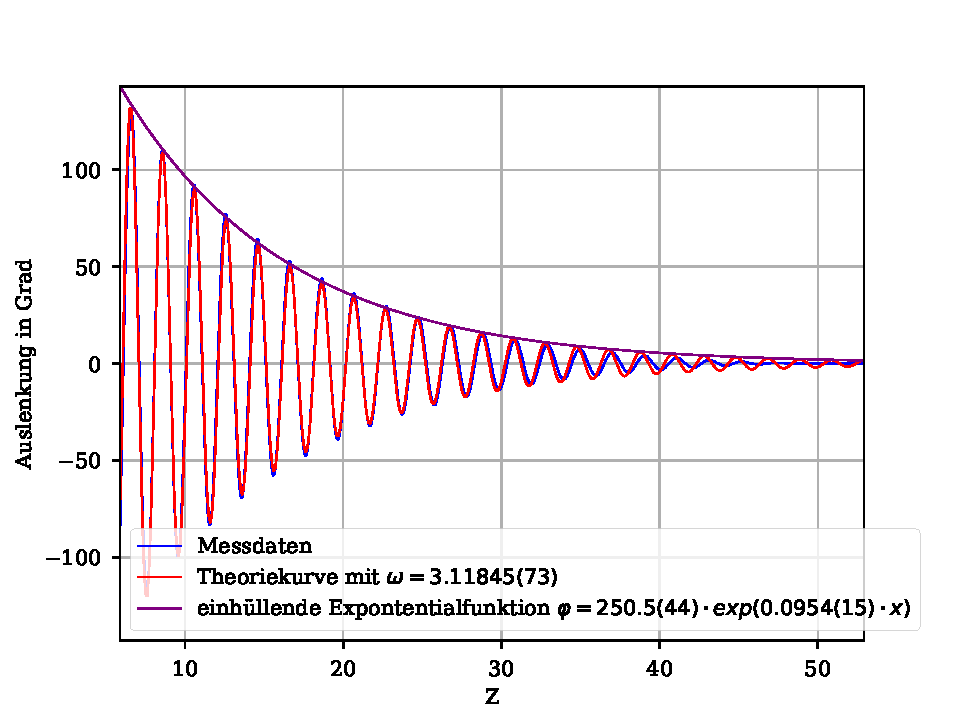
\includegraphics[width=\textwidth]{./8comp.pdf}

        \caption{Messung der Eigenfrequenz}
        \label{fig:eigenfrequenz}
    \end{figure}
    \begin{figure}
        \centering
        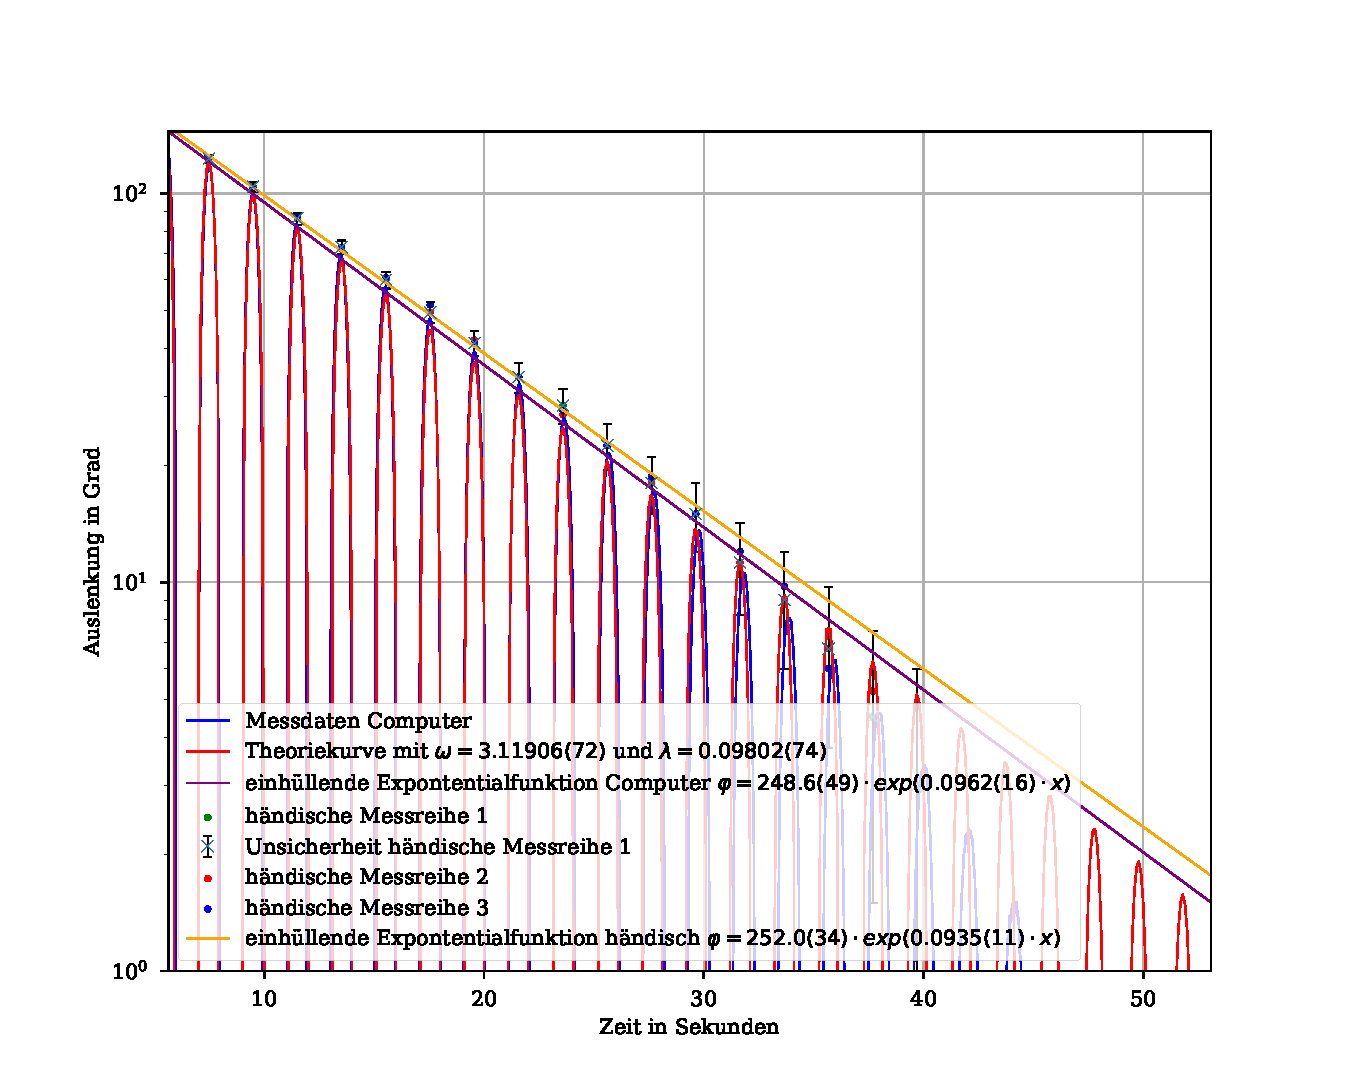
\includegraphics[width=\textwidth]{./9all.pdf}

        \caption{Messung der Dämpfungskonstante}
        \label{fig:daempfung}
    \end{figure}
    In Graph \ref{fig:eigenfrequenz} kann die digitale Messung und die gefittete
    Funktion gesehen werden. Die gleiche einhüllende Exponentialfunktion sowie die Daten der händischen Amplitudenmessung
    wurden im Graphen \ref{fig:daempfung} halblogarithmisch dargestellt.
    
    Als Fehler wurden bei der händischen Messung der Eigenfrequenz berücksichtigt, die Ungenauigkeit der Stoppuhr hingegen
    wurde vernachlässigt, da sie um Größenordnungen kleiner ist. Bei der Amplitudenmessung wird eine Unsicherheit von ca. 2 Strichen
    oder $3^{\circ}$ angenommen, da die Daten schnell abgelesen werden müssen.
    In Tabelle \ref{Tab:tableeig} wird die händisch gemessene Dämpfungskonstante und Eigenfrequenz (Herleitung siehe Anhang \ref{sec:omega}) sowie die
    digital gemessene Dämpfungskonstante und Eigenfrequenz angegeben. 
    \begin{table}[H]
        \centering
        \begin{tabular}{c c c} 
            & Hand & Computer \\ \hline
            Eigenfrequenz $\omega$ & $3,118(24) \si{\radian\per\second}$ & $3.11913(74) \si{\radian\per\second}$ \\
            Dämpfungskonstante $\lambda$ & $0,0935(11) \si{\per\second}$ & $0.0962(16) \si{\per\second}$ \\
            Abklingzeit $\tau$ & 10,70(13) \si{\second} & 10,40(17) \si{\second} \\

            
        \end{tabular}
        \caption{Eigenfrequenz im Vergleich}
        \label{Tab:tableeig}
    \end{table}

	\subsubsection{Resonanzkurve}

	\begin{figure}[h]
        \centering
        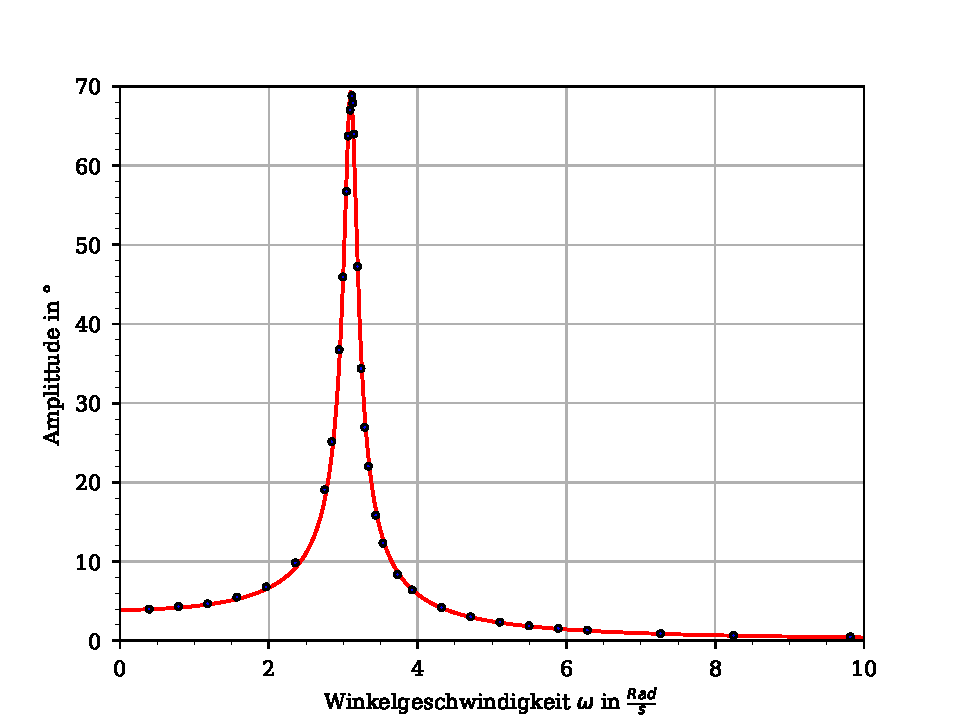
\includegraphics[width=\textwidth]{./10Plot.pdf}

        \caption{Resonanzkurve}
        \label{fig:Resonanzkurve}
    \end{figure}
    In \ref{fig:Resonanzkurve} werden die Amplituden in Bezug zu ihrer Anregungsfrequenz aufgetragen, die Messdaten sind
    mit der Theoriekurve \ref{aomega} gefittet. Dabei sind die Fehler der einzelnen Messdaten zu klein um sie in \ref{fig:Resonanzkurve}
    sinnvoll darstellen zu können. Aus dem Fit ergibt sich eine Eigenfrequenz von $\omega_0=3.1030(15) \si{\radian\per\second}$, eine Dämpfungskonstante
    von $\lambda=0.0877(18) \si{\per\second}$. Durch Berechnung der Extremstellen an der gefitteten Funktion \ref{fig:Resonanzkurve} konnte eine Resonanzfrequenz
    von $\omega_R=3.10054 \si{\radian\per\second}$ bestimmt werden und somit eine Maximale Amplitude von $A(\omega_R)=69.287 \si{\degree}$.
    Die Halbwertsbreite beträg $2\lambda=0.175 \si{\per\second}$ und liegt somit im Fehlerintervall vom $\lambda$
	
    \section{Diskussion}

    Man merkt bei den Fits, dass das Pohlsche Rad nicht genau der Theoriekurve folgt, sondern das bei kleinen Anplituden
    weitere Effekte, die wahrscheinlich nicht durch die gedämpft harmonische Schwingung beschrieben können, beobachtet werden können.
    So gibt es immer Abweichungen bei kleineren Amplituden, die den Fehler des Fits vergrößern. Wahrscheinlich exixtieren noch weitere
    Reibungskräfte im Lager des Pohlschen Rades. \\

    Obwohl keine Literaturwerte vorhanden sind, kann davon ausgegangen werden, dass die bestimmten Werte realistisch sind.
    Bei allen Kurven außer der Graph \ref{fig:wink} liegt die Theoriekurve in der Fehlertoleranz der einzelnen Messungen.
    Bei der Berechnung der Dämpfungkonstante überschneiden sich die Unsicherheiten der Messungen von Computer und per Hand,
    jedoch nur so  wenig, dass bei einer Messung wahrscheinlich das Konfidenzintervall zu klein gewählt wurde. Bei der
    Berechnung der Eigenfrequenz hingegen, sind die Messungen sehr nahe bei einander. Auffällig ist, dass war wie zu
    erwarten bei der Eigenfrequenz die Unsicherheit per Hand um eine Größenordnung größer als beim Computer ist,
    aber bei der Dämpfungskonstanten die Unischerheit der Computermessung etwas größer ist. Dies liegt wahrscheinlich an der Anfangs
    erwähnten Diskrepanz zwischen Theorie und Praxis.

    \section{Anhang}

    \subsection{Berechnung von Omega und Fehlerfortpflanzung} \label{sec:omega}
    Zur Berechnung von $\omega_d$ wurden 5 Messungen von 10 Schwingungen duchgeführt.
    \begin{table}
        \centering
        \begin{tabular}{c c}
            Messung & Zeit in Sekunden \\ \hline
            1 & 20,24 \\
            2 & 20,30 \\
            3 & 20,09 \\
            4 & 20,08 \\
            5 & 20,04
        \end{tabular}
        \caption{Messung Schwingungsdauer}
        \label{Tab:messen}
    \end{table}
    von diesen wurde der Mittelwert berechnet. Um dann mit der Gauschen Fehlerfortpflanzung \cite[(19)]{ABW} $\omega_d$ zu berechnen.
    \begin{align}
        \bar{t} &= \frac{1}{5} \left(20,24 + 20,30 + 20,09 + 20,08 + 20,04 \right) \si{\second} = 20.15 \\
        u(t_n) &= 0,3 \si{\second} \text{Reaktionszeit} \\
        u(\bar{t}) &= \frac{{\it t}}{\sqrt{n}} u(t_n) = 0.153 \si{\second} \text{Student-t} \\
        \text{Zeit für eine Schwingung: } \ \ T &= \frac{10}{\bar{t}} \\
        u(\omega) &= \frac{2 \pi \cdot 10}{\bar{t}} \cdot u(\bar{t}) = 0,0237 \si{\radian\per\second} \\
        \omega_d &= 2 \pi \cdot \frac{10}{\bar{t}} = 3.118(24) \si{\radian\per\second}
        \tau &= frac{1}{\lambda} \\
        u(\tau) &= \frac{1}{\lambda^2} \cdot u(\lambda)
    \end{align}


    \bibliographystyle{plain}
    \bibliography{literature}

\end{document}